\chapter{Clustering Analysis (CA)} 
%\bibliographystyle{nar}
\label{appendix_a}

\section{Hierarchical methods}
The hierarchical clustering methods used were:

\begin{enumerate}
\item{
\textit{Single linkage clustering}, where the minimum distance between
elements of each cluster is taken as clustering criteria.
\begin{gather}
D(X, Y)=min\{d(x_i, y_j): x_i \in X, y_j \in Y \}
\end{gather}
where $X$ and $Y$ are vectors, and $d(x_i, y_j)$ is the distance
between cluster elements.
}

\item{
\textit{Complete linkage clustering}, where the maximum distance between
cluster elements is the clustering criteria.
\begin{gather}
D(X, Y)=max\{d(x_i, y_j): x_i \in X, y_j \in Y \}
\end{gather}
}

\item{
\textit{Average linkage clustering}, the mean distance between elements of
each cluster is taken as clustering criteria.
\begin{gather}
D(X, Y)=\frac{1}{N_x * N_y} \sum_{i=1}^{N_x} \sum_{j=1}^{N_y} d(x_i, y_j)
\end{gather}
where $N_x$ and $N_y$ are the number of elements in respective clusters.
}

\item{
\textit{Centroid linkage clustering}, uses the distance between cluster
centroids, as clustering criteria.
\begin{gather}
D(X, Y)=d(\overline{x}, \overline{y})\\
\overline{x} = \frac{1}{N_x} \sum_{i=1}^{N_x} x_i\\
\overline{y} = \frac{1}{N_y} \sum_{i=1}^{N_y} y_i\\
\end{gather}
}

\item{
\textit{Ward's Method}, uses the error sum of squares (ESS).
%This Error Sum of Squares might be the same as the residual sum of squares
%which is important in regression models.
\begin{gather}
D(X,Y)=ESS(XY) -[ESS(X) + ESS(Y)]\\
ESS(X)= \sum_{i=1}^{N_x} \left| x_i -\frac{1}{N_x}\sum_{j=1}^{N_x} x_j\right|^2
\end{gather}
}
\end{enumerate}




As an example lets think of a case where we have five structures. Each one
of them is descibed by a bidimensional vector as illustrated in
Table~\ref{tab:data}.
\begin{table}
\centering
\begin{tabular}[h]{|c|c|c|}
\hline
Structure & Property I & Property II\\
\hline\hline
1  &     1.00  &  5.00 \\
\hline
2  &    -2.00  & 6.00 \\
\hline
3  &      2.00  & -2.00 \\
\hline
4  &     -2.00  & -3.00 \\
\hline
5  &     3.00  &  -4.00 \\
\hline
\end{tabular}
\caption{Example of structures, considered as bidimensional vectors, to be
clustered using the average linkage method and the Manhattan distance.}
\label{tab:data}
\end{table}

The first step is to chose a distance definition. We chose Manhattan and the
distance values between structures can be displayed in a lower triangular
matrix as seen in equation~\ref{eq:man}
\begin{gather} 
d(X, Y)=
\begin{vmatrix}
    & 1  &  2   & 3 & 4 \\
1  &     &       &    &     \\
2  & 4  &       &    &     \\
3  & 8  & 12 &    &      \\
4  & 11 &  9  & 5 &      \\
5  & 11 & 15 & 3 & 6 \\
\end{vmatrix}
\label{eq:man}
\end{gather}

Let's calculate explicitily the Manhattan distance between structures 2 and 3,

\begin{gather}
d(2, 3)= |-2.00 - 6.00| + |2.00 - -2.00| = 12
\end{gather}

Now that we have calculated the distances we need a clustering method, in this
case, we will use the average linkage clustering method. The first step is to
group whatever structures are closer, that is, structures 3 and 5
($d(3, 5)=3$). Now we find the mean distance between the elements of
this cluster and the remaining unclustered structures, that is,
structures 1, 2 and 4, we obtain the following mean distances
\begin{gather}
D(\{3,5\}, 1)=\frac{1}{2*1}*(8+11) = 4.5 \label{eq:dist}\\
D(\{3,5\}, 2)=\frac{1}{2*1}*(12+15) = 13.5\\
D(\{3,5\}, 4)=\frac{1}{2*1}*(5+6) = 5.5
\end{gather}
Since the distances between \{3, 5\} and all remaining unclustered
vectors is higher than the distance between vectors 1 and 2
($d(1, 2)=4$) then \{1, 2\} are grouped. The following value, in
hierarchical increasing order is 4.5 between \{3, 5\} and 1 (see
equation~\ref{eq:dist}), but since 1 and 2 are already
grouped we can't group \{3, 5\} with 1. The next value,
following the lower to higher hierarchy, is 5 ($d(3, 4)=5$), but we have
already grouped 3 with 5, so we have to keep advancing in the
hierarchy. The next value is 5.5, which corresponds to grouping \{3,
5\} with 4, so we cluster them. The only remaining possibility for
grouping is, group \{1, 2\} and \{4, 3, 5\}, so we do it as
illustrated in Figure~\ref{fig:tree}.
\begin{figure}[t]
\centering
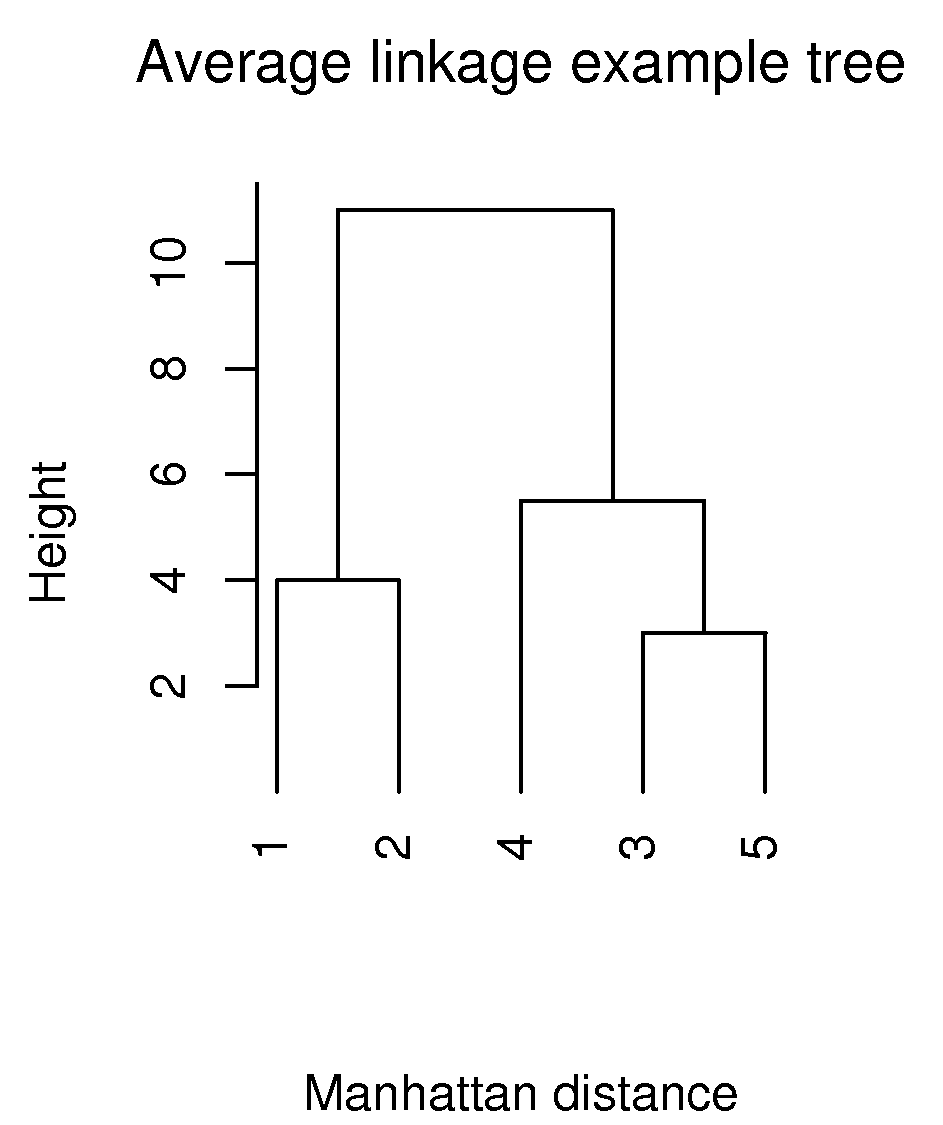
\includegraphics[scale=0.4]{appendixtree.png}
\caption{Clustering tree for 5 bidimensional vectors using the Manhattan
distance definition and the average linkage clustering method.}
\label{fig:tree}
\end{figure}


%\newline
%Distance can be defined by Minkowski's metric:
%\begin{gather}
%d(X,Y)= \Big( \sum_{i=1}^N |x_i-y_i|^k \Big)^\frac{1}{k}
%\end{gather}
%In the particular case when $k=1$ we have the definition of the
%Manhattan or taxi-cab distance and when $k=2$ it's the familiar
%Euclidean distance.

%Finally, we can also define a maximum distance as the maximum
%difference between vectors variables.
%\begin{gather}
%d(X,Y) = max |x_{i}-y_{i}|
%\end{gather}

%\bibliography{biblio}


